\documentclass[twoside]{book}

% Packages required by doxygen
\usepackage{fixltx2e}
\usepackage{calc}
\usepackage{doxygen}
\usepackage[export]{adjustbox} % also loads graphicx
\usepackage{graphicx}
\usepackage[utf8]{inputenc}
\usepackage{makeidx}
\usepackage{multicol}
\usepackage{multirow}
\PassOptionsToPackage{warn}{textcomp}
\usepackage{textcomp}
\usepackage[nointegrals]{wasysym}
\usepackage[table]{xcolor}

% Font selection
\usepackage[T1]{fontenc}
\usepackage[scaled=.90]{helvet}
\usepackage{courier}
\usepackage{amssymb}
\usepackage{sectsty}
\renewcommand{\familydefault}{\sfdefault}
\allsectionsfont{%
  \fontseries{bc}\selectfont%
  \color{darkgray}%
}
\renewcommand{\DoxyLabelFont}{%
  \fontseries{bc}\selectfont%
  \color{darkgray}%
}
\newcommand{\+}{\discretionary{\mbox{\scriptsize$\hookleftarrow$}}{}{}}

% Page & text layout
\usepackage{geometry}
\geometry{%
  a4paper,%
  top=2.5cm,%
  bottom=2.5cm,%
  left=2.5cm,%
  right=2.5cm%
}
\tolerance=750
\hfuzz=15pt
\hbadness=750
\setlength{\emergencystretch}{15pt}
\setlength{\parindent}{0cm}
\setlength{\parskip}{3ex plus 2ex minus 2ex}
\makeatletter
\renewcommand{\paragraph}{%
  \@startsection{paragraph}{4}{0ex}{-1.0ex}{1.0ex}{%
    \normalfont\normalsize\bfseries\SS@parafont%
  }%
}
\renewcommand{\subparagraph}{%
  \@startsection{subparagraph}{5}{0ex}{-1.0ex}{1.0ex}{%
    \normalfont\normalsize\bfseries\SS@subparafont%
  }%
}
\makeatother

% Headers & footers
\usepackage{fancyhdr}
\pagestyle{fancyplain}
\fancyhead[LE]{\fancyplain{}{\bfseries\thepage}}
\fancyhead[CE]{\fancyplain{}{}}
\fancyhead[RE]{\fancyplain{}{\bfseries\leftmark}}
\fancyhead[LO]{\fancyplain{}{\bfseries\rightmark}}
\fancyhead[CO]{\fancyplain{}{}}
\fancyhead[RO]{\fancyplain{}{\bfseries\thepage}}
\fancyfoot[LE]{\fancyplain{}{}}
\fancyfoot[CE]{\fancyplain{}{}}
\fancyfoot[RE]{\fancyplain{}{\bfseries\scriptsize Generated by Doxygen }}
\fancyfoot[LO]{\fancyplain{}{\bfseries\scriptsize Generated by Doxygen }}
\fancyfoot[CO]{\fancyplain{}{}}
\fancyfoot[RO]{\fancyplain{}{}}
\renewcommand{\footrulewidth}{0.4pt}
\renewcommand{\chaptermark}[1]{%
  \markboth{#1}{}%
}
\renewcommand{\sectionmark}[1]{%
  \markright{\thesection\ #1}%
}

% Indices & bibliography
\usepackage{natbib}
\usepackage[titles]{tocloft}
\setcounter{tocdepth}{3}
\setcounter{secnumdepth}{5}
\makeindex

% Hyperlinks (required, but should be loaded last)
\usepackage{ifpdf}
\ifpdf
  \usepackage[pdftex,pagebackref=true]{hyperref}
\else
  \usepackage[ps2pdf,pagebackref=true]{hyperref}
\fi
\hypersetup{%
  colorlinks=true,%
  linkcolor=blue,%
  citecolor=blue,%
  unicode%
}

% Custom commands
\newcommand{\clearemptydoublepage}{%
  \newpage{\pagestyle{empty}\cleardoublepage}%
}

\usepackage{caption}
\captionsetup{labelsep=space,justification=centering,font={bf},singlelinecheck=off,skip=4pt,position=top}

%===== C O N T E N T S =====

\begin{document}

% Titlepage & ToC
\hypersetup{pageanchor=false,
             bookmarksnumbered=true,
             pdfencoding=unicode
            }
\pagenumbering{alph}
\begin{titlepage}
\vspace*{7cm}
\begin{center}%
{\Large D\+MA for U\+C\+AS \\[1ex]\large 0.\+1.\+0 }\\
\vspace*{1cm}
{\large Generated by Doxygen 1.8.15}\\
\end{center}
\end{titlepage}
\clearemptydoublepage
\pagenumbering{roman}
\tableofcontents
\clearemptydoublepage
\pagenumbering{arabic}
\hypersetup{pageanchor=true}

%--- Begin generated contents ---
\chapter{Hierarchical Index}
\section{Class Hierarchy}
This inheritance list is sorted roughly, but not completely, alphabetically\+:\begin{DoxyCompactList}
\item \contentsline{section}{fifo}{\pageref{enumfifo}}{}
\begin{DoxyCompactList}
\item \contentsline{section}{dma}{\pageref{enumdma}}{}
\end{DoxyCompactList}
\end{DoxyCompactList}

\chapter{Class Index}
\section{Class List}
Here are the classes, structs, unions and interfaces with brief descriptions\+:\begin{DoxyCompactList}
\item\contentsline{section}{\mbox{\hyperlink{enumdma}{dma}} }{\pageref{enumdma}}{}
\item\contentsline{section}{\mbox{\hyperlink{enumfifo}{fifo}} }{\pageref{enumfifo}}{}
\end{DoxyCompactList}

\chapter{File Index}
\section{File List}
Here is a list of all files with brief descriptions\+:\begin{DoxyCompactList}
\item\contentsline{section}{Final\+Elec.\+srcs/sources\+\_\+1/new/\mbox{\hyperlink{dma_8v}{dma.\+v}} }{\pageref{dma_8v}}{}
\item\contentsline{section}{Final\+Elec.\+srcs/sources\+\_\+1/new/\mbox{\hyperlink{fifo_8v}{fifo.\+v}} \\*First in first out memory module }{\pageref{fifo_8v}}{}
\end{DoxyCompactList}

\chapter{Class Documentation}
\hypertarget{enumdma}{}\section{dma Module Reference}
\label{enumdma}\index{dma@{dma}}
Inheritance diagram for dma\+:\begin{figure}[H]
\begin{center}
\leavevmode
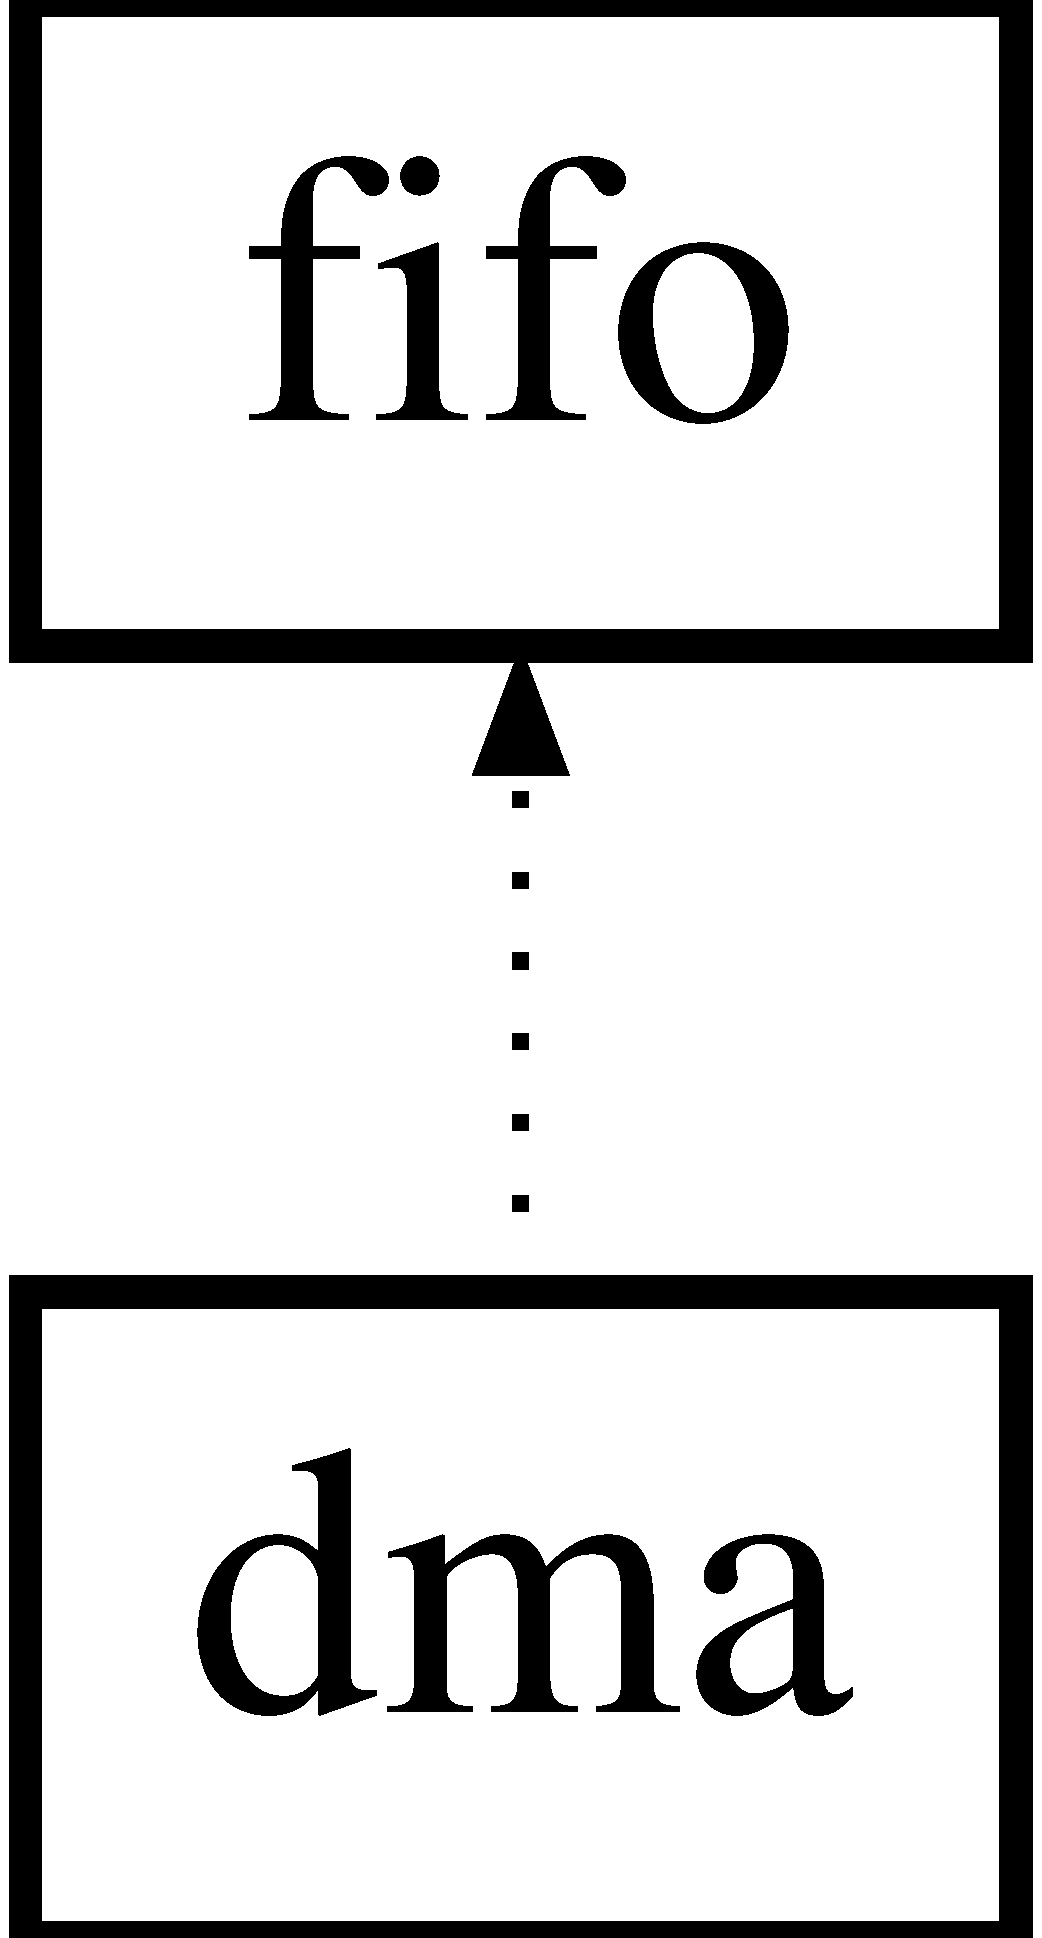
\includegraphics[height=2.000000cm]{d2/d5b/enumdma}
\end{center}
\end{figure}
\begin{DoxyCompactItemize}
\item 
\mbox{\hyperlink{enumdma_a0481abb8206ba22fcd1bad5db283afd1}{clk}}
\item 
\mbox{\hyperlink{enumdma_a18bc13bcbec8196090081641b8de9113}{rst}}
\item 
\mbox{\hyperlink{enumdma_aac28a8c8df33b5bcce79447347957a72}{dir}}
\item 
\mbox{\hyperlink{enumdma_a1378adba2e74daaf6d8f4e2a0a15c512}{float\+\_\+direction}}
\item 
\mbox{\hyperlink{enumdma_a1187ad902d0d07b25c4dfe7fb099a45e}{mem\+\_\+to\+\_\+dma\+\_\+valid}}
\item 
\mbox{\hyperlink{enumdma_a2269f9e84b5c4626b6153a5a37065f90}{mem\+\_\+to\+\_\+dma\+\_\+enable}}
\item 
\mbox{\hyperlink{enumdma_a6fabf91cc2d29bb39c4ec91bce8880ff}{cpu\+\_\+to\+\_\+dma\+\_\+valid}}
\item 
\mbox{\hyperlink{enumdma_a8693a930e7a23b7cff186909af9df454}{cpu\+\_\+to\+\_\+dma\+\_\+enable}}
\item 
\mbox{\hyperlink{enumdma_adebb6c45028d9e8abd6919e9b6dc6492}{dma\+\_\+to\+\_\+mem\+\_\+valid}}
\item 
\mbox{\hyperlink{enumdma_a272e3d64b1ec70497ac14bd358a6e976}{dma\+\_\+to\+\_\+mem\+\_\+enable}}
\item 
\mbox{\hyperlink{enumdma_afe45981e0efd23c51407c4ce3c4ee37e}{dma\+\_\+to\+\_\+cpu\+\_\+valid}}
\item 
\mbox{\hyperlink{enumdma_ac8f125b33d488e6f6113171199a9de9d}{dma\+\_\+to\+\_\+cpu\+\_\+enable}}
\item 
\mbox{[}3\+:0\mbox{]} \mbox{\hyperlink{enumdma_a04109ea4541b06cba36bc5b2d7427d0d}{mem\+\_\+data\+\_\+out}}
\item 
\mbox{[}7\+:0\mbox{]} \mbox{\hyperlink{enumdma_a63dd3df5324f66dc3f1c60bf5999ef29}{cpu\+\_\+data\+\_\+out}}
\item 
reg \mbox{[}3\+:0\mbox{]} \mbox{\hyperlink{enumdma_a9915f2241fbb74c3f70857b53e7b7d71}{mem\+\_\+data\+\_\+in}}
\item 
reg \mbox{[}7\+:0\mbox{]} \mbox{\hyperlink{enumdma_a30462d21c7a22410c6f1dfda0c47c1a0}{cpu\+\_\+data\+\_\+in}}
\item 
buffer\+\_\+cpu\+\_\+to\+\_\+mem \mbox{\hyperlink{enumdma_aae0a35ee18bd585d93077404ec59bb29}{fifo}}
\item 
\mbox{\hyperlink{enumdma_a6960126d1f81033b251f52fa60128d67}{buffer\+\_\+valid\+\_\+cpu\+\_\+to\+\_\+mem}} reg\mbox{[}2\+:0\mbox{]}
\item 
\mbox{\hyperlink{enumdma_a99a56ad3a0ba7758b4e47e1c598610b9}{buffer\+\_\+valid\+\_\+mem\+\_\+to\+\_\+cpu}} reg\mbox{[}2\+:0\mbox{]}
\item 
\mbox{\hyperlink{enumdma_a5f20405a60143989302bdabc9d9f4fa6}{buffer\+\_\+empty\+\_\+cpu\+\_\+to\+\_\+mem}} reg
\item 
\mbox{\hyperlink{enumdma_ad59cb5889c658ccad5feda1cdc17f839}{buffer\+\_\+empty\+\_\+mem\+\_\+to\+\_\+cpu}} reg
\end{DoxyCompactItemize}


\subsection{Member Data Documentation}
\mbox{\Hypertarget{enumdma_a0481abb8206ba22fcd1bad5db283afd1}\label{enumdma_a0481abb8206ba22fcd1bad5db283afd1}} 
\index{dma@{dma}!clk@{clk}}
\index{clk@{clk}!dma@{dma}}
\subsubsection{\texorpdfstring{clk}{clk}}
{\footnotesize\ttfamily \mbox{\hyperlink{enumdma_a0481abb8206ba22fcd1bad5db283afd1}{clk}} \hspace{0.3cm}{\ttfamily [Input]}}

\mbox{\Hypertarget{enumdma_afe45981e0efd23c51407c4ce3c4ee37e}\label{enumdma_afe45981e0efd23c51407c4ce3c4ee37e}} 
\index{dma@{dma}!dma\+\_\+to\+\_\+cpu\+\_\+valid@{dma\+\_\+to\+\_\+cpu\+\_\+valid}}
\index{dma\+\_\+to\+\_\+cpu\+\_\+valid@{dma\+\_\+to\+\_\+cpu\+\_\+valid}!dma@{dma}}
\subsubsection{\texorpdfstring{dma\+\_\+to\+\_\+cpu\+\_\+valid}{dma\_to\_cpu\_valid}}
{\footnotesize\ttfamily \mbox{\hyperlink{enumdma_afe45981e0efd23c51407c4ce3c4ee37e}{dma\+\_\+to\+\_\+cpu\+\_\+valid}} \hspace{0.3cm}{\ttfamily [Output]}}

\mbox{\Hypertarget{enumdma_ac8f125b33d488e6f6113171199a9de9d}\label{enumdma_ac8f125b33d488e6f6113171199a9de9d}} 
\index{dma@{dma}!dma\+\_\+to\+\_\+cpu\+\_\+enable@{dma\+\_\+to\+\_\+cpu\+\_\+enable}}
\index{dma\+\_\+to\+\_\+cpu\+\_\+enable@{dma\+\_\+to\+\_\+cpu\+\_\+enable}!dma@{dma}}
\subsubsection{\texorpdfstring{dma\+\_\+to\+\_\+cpu\+\_\+enable}{dma\_to\_cpu\_enable}}
{\footnotesize\ttfamily \mbox{\hyperlink{enumdma_ac8f125b33d488e6f6113171199a9de9d}{dma\+\_\+to\+\_\+cpu\+\_\+enable}} \hspace{0.3cm}{\ttfamily [Output]}}

\mbox{\Hypertarget{enumdma_a04109ea4541b06cba36bc5b2d7427d0d}\label{enumdma_a04109ea4541b06cba36bc5b2d7427d0d}} 
\index{dma@{dma}!mem\+\_\+data\+\_\+out@{mem\+\_\+data\+\_\+out}}
\index{mem\+\_\+data\+\_\+out@{mem\+\_\+data\+\_\+out}!dma@{dma}}
\subsubsection{\texorpdfstring{mem\+\_\+data\+\_\+out}{mem\_data\_out}}
{\footnotesize\ttfamily \mbox{\hyperlink{enumdma_a04109ea4541b06cba36bc5b2d7427d0d}{mem\+\_\+data\+\_\+out}} \hspace{0.3cm}{\ttfamily [Input]}}

\mbox{\Hypertarget{enumdma_a63dd3df5324f66dc3f1c60bf5999ef29}\label{enumdma_a63dd3df5324f66dc3f1c60bf5999ef29}} 
\index{dma@{dma}!cpu\+\_\+data\+\_\+out@{cpu\+\_\+data\+\_\+out}}
\index{cpu\+\_\+data\+\_\+out@{cpu\+\_\+data\+\_\+out}!dma@{dma}}
\subsubsection{\texorpdfstring{cpu\+\_\+data\+\_\+out}{cpu\_data\_out}}
{\footnotesize\ttfamily \mbox{\hyperlink{enumdma_a63dd3df5324f66dc3f1c60bf5999ef29}{cpu\+\_\+data\+\_\+out}} \hspace{0.3cm}{\ttfamily [Input]}}

\mbox{\Hypertarget{enumdma_a9915f2241fbb74c3f70857b53e7b7d71}\label{enumdma_a9915f2241fbb74c3f70857b53e7b7d71}} 
\index{dma@{dma}!mem\+\_\+data\+\_\+in@{mem\+\_\+data\+\_\+in}}
\index{mem\+\_\+data\+\_\+in@{mem\+\_\+data\+\_\+in}!dma@{dma}}
\subsubsection{\texorpdfstring{mem\+\_\+data\+\_\+in}{mem\_data\_in}}
{\footnotesize\ttfamily \mbox{\hyperlink{enumdma_a9915f2241fbb74c3f70857b53e7b7d71}{mem\+\_\+data\+\_\+in}} \hspace{0.3cm}{\ttfamily [Output]}}

\mbox{\Hypertarget{enumdma_a30462d21c7a22410c6f1dfda0c47c1a0}\label{enumdma_a30462d21c7a22410c6f1dfda0c47c1a0}} 
\index{dma@{dma}!cpu\+\_\+data\+\_\+in@{cpu\+\_\+data\+\_\+in}}
\index{cpu\+\_\+data\+\_\+in@{cpu\+\_\+data\+\_\+in}!dma@{dma}}
\subsubsection{\texorpdfstring{cpu\+\_\+data\+\_\+in}{cpu\_data\_in}}
{\footnotesize\ttfamily \mbox{\hyperlink{enumdma_a30462d21c7a22410c6f1dfda0c47c1a0}{cpu\+\_\+data\+\_\+in}} \hspace{0.3cm}{\ttfamily [Output]}}

\mbox{\Hypertarget{enumdma_a6960126d1f81033b251f52fa60128d67}\label{enumdma_a6960126d1f81033b251f52fa60128d67}} 
\index{dma@{dma}!buffer\+\_\+valid\+\_\+cpu\+\_\+to\+\_\+mem@{buffer\+\_\+valid\+\_\+cpu\+\_\+to\+\_\+mem}}
\index{buffer\+\_\+valid\+\_\+cpu\+\_\+to\+\_\+mem@{buffer\+\_\+valid\+\_\+cpu\+\_\+to\+\_\+mem}!dma@{dma}}
\subsubsection{\texorpdfstring{buffer\+\_\+valid\+\_\+cpu\+\_\+to\+\_\+mem}{buffer\_valid\_cpu\_to\_mem}}
{\footnotesize\ttfamily \mbox{\hyperlink{enumdma_a6960126d1f81033b251f52fa60128d67}{buffer\+\_\+valid\+\_\+cpu\+\_\+to\+\_\+mem}} \hspace{0.3cm}{\ttfamily [Signal]}}

\mbox{\Hypertarget{enumdma_a99a56ad3a0ba7758b4e47e1c598610b9}\label{enumdma_a99a56ad3a0ba7758b4e47e1c598610b9}} 
\index{dma@{dma}!buffer\+\_\+valid\+\_\+mem\+\_\+to\+\_\+cpu@{buffer\+\_\+valid\+\_\+mem\+\_\+to\+\_\+cpu}}
\index{buffer\+\_\+valid\+\_\+mem\+\_\+to\+\_\+cpu@{buffer\+\_\+valid\+\_\+mem\+\_\+to\+\_\+cpu}!dma@{dma}}
\subsubsection{\texorpdfstring{buffer\+\_\+valid\+\_\+mem\+\_\+to\+\_\+cpu}{buffer\_valid\_mem\_to\_cpu}}
{\footnotesize\ttfamily \mbox{\hyperlink{enumdma_a99a56ad3a0ba7758b4e47e1c598610b9}{buffer\+\_\+valid\+\_\+mem\+\_\+to\+\_\+cpu}} \hspace{0.3cm}{\ttfamily [Signal]}}

\mbox{\Hypertarget{enumdma_a5f20405a60143989302bdabc9d9f4fa6}\label{enumdma_a5f20405a60143989302bdabc9d9f4fa6}} 
\index{dma@{dma}!buffer\+\_\+empty\+\_\+cpu\+\_\+to\+\_\+mem@{buffer\+\_\+empty\+\_\+cpu\+\_\+to\+\_\+mem}}
\index{buffer\+\_\+empty\+\_\+cpu\+\_\+to\+\_\+mem@{buffer\+\_\+empty\+\_\+cpu\+\_\+to\+\_\+mem}!dma@{dma}}
\subsubsection{\texorpdfstring{buffer\+\_\+empty\+\_\+cpu\+\_\+to\+\_\+mem}{buffer\_empty\_cpu\_to\_mem}}
{\footnotesize\ttfamily \mbox{\hyperlink{enumdma_a5f20405a60143989302bdabc9d9f4fa6}{buffer\+\_\+empty\+\_\+cpu\+\_\+to\+\_\+mem}} \hspace{0.3cm}{\ttfamily [Signal]}}

\mbox{\Hypertarget{enumdma_ad59cb5889c658ccad5feda1cdc17f839}\label{enumdma_ad59cb5889c658ccad5feda1cdc17f839}} 
\index{dma@{dma}!buffer\+\_\+empty\+\_\+mem\+\_\+to\+\_\+cpu@{buffer\+\_\+empty\+\_\+mem\+\_\+to\+\_\+cpu}}
\index{buffer\+\_\+empty\+\_\+mem\+\_\+to\+\_\+cpu@{buffer\+\_\+empty\+\_\+mem\+\_\+to\+\_\+cpu}!dma@{dma}}
\subsubsection{\texorpdfstring{buffer\+\_\+empty\+\_\+mem\+\_\+to\+\_\+cpu}{buffer\_empty\_mem\_to\_cpu}}
{\footnotesize\ttfamily \mbox{\hyperlink{enumdma_ad59cb5889c658ccad5feda1cdc17f839}{buffer\+\_\+empty\+\_\+mem\+\_\+to\+\_\+cpu}} \hspace{0.3cm}{\ttfamily [Signal]}}

\mbox{\Hypertarget{enumdma_a18bc13bcbec8196090081641b8de9113}\label{enumdma_a18bc13bcbec8196090081641b8de9113}} 
\index{dma@{dma}!rst@{rst}}
\index{rst@{rst}!dma@{dma}}
\subsubsection{\texorpdfstring{rst}{rst}}
{\footnotesize\ttfamily \mbox{\hyperlink{enumdma_a18bc13bcbec8196090081641b8de9113}{rst}} \hspace{0.3cm}{\ttfamily [Input]}}

\mbox{\Hypertarget{enumdma_aac28a8c8df33b5bcce79447347957a72}\label{enumdma_aac28a8c8df33b5bcce79447347957a72}} 
\index{dma@{dma}!dir@{dir}}
\index{dir@{dir}!dma@{dma}}
\subsubsection{\texorpdfstring{dir}{dir}}
{\footnotesize\ttfamily \mbox{\hyperlink{enumdma_aac28a8c8df33b5bcce79447347957a72}{dir}} \hspace{0.3cm}{\ttfamily [Input]}}

\mbox{\Hypertarget{enumdma_a1378adba2e74daaf6d8f4e2a0a15c512}\label{enumdma_a1378adba2e74daaf6d8f4e2a0a15c512}} 
\index{dma@{dma}!float\+\_\+direction@{float\+\_\+direction}}
\index{float\+\_\+direction@{float\+\_\+direction}!dma@{dma}}
\subsubsection{\texorpdfstring{float\+\_\+direction}{float\_direction}}
{\footnotesize\ttfamily \mbox{\hyperlink{enumdma_a1378adba2e74daaf6d8f4e2a0a15c512}{float\+\_\+direction}} \hspace{0.3cm}{\ttfamily [Input]}}

\mbox{\Hypertarget{enumdma_a1187ad902d0d07b25c4dfe7fb099a45e}\label{enumdma_a1187ad902d0d07b25c4dfe7fb099a45e}} 
\index{dma@{dma}!mem\+\_\+to\+\_\+dma\+\_\+valid@{mem\+\_\+to\+\_\+dma\+\_\+valid}}
\index{mem\+\_\+to\+\_\+dma\+\_\+valid@{mem\+\_\+to\+\_\+dma\+\_\+valid}!dma@{dma}}
\subsubsection{\texorpdfstring{mem\+\_\+to\+\_\+dma\+\_\+valid}{mem\_to\_dma\_valid}}
{\footnotesize\ttfamily \mbox{\hyperlink{enumdma_a1187ad902d0d07b25c4dfe7fb099a45e}{mem\+\_\+to\+\_\+dma\+\_\+valid}} \hspace{0.3cm}{\ttfamily [Input]}}

\mbox{\Hypertarget{enumdma_a2269f9e84b5c4626b6153a5a37065f90}\label{enumdma_a2269f9e84b5c4626b6153a5a37065f90}} 
\index{dma@{dma}!mem\+\_\+to\+\_\+dma\+\_\+enable@{mem\+\_\+to\+\_\+dma\+\_\+enable}}
\index{mem\+\_\+to\+\_\+dma\+\_\+enable@{mem\+\_\+to\+\_\+dma\+\_\+enable}!dma@{dma}}
\subsubsection{\texorpdfstring{mem\+\_\+to\+\_\+dma\+\_\+enable}{mem\_to\_dma\_enable}}
{\footnotesize\ttfamily \mbox{\hyperlink{enumdma_a2269f9e84b5c4626b6153a5a37065f90}{mem\+\_\+to\+\_\+dma\+\_\+enable}} \hspace{0.3cm}{\ttfamily [Input]}}

\mbox{\Hypertarget{enumdma_a6fabf91cc2d29bb39c4ec91bce8880ff}\label{enumdma_a6fabf91cc2d29bb39c4ec91bce8880ff}} 
\index{dma@{dma}!cpu\+\_\+to\+\_\+dma\+\_\+valid@{cpu\+\_\+to\+\_\+dma\+\_\+valid}}
\index{cpu\+\_\+to\+\_\+dma\+\_\+valid@{cpu\+\_\+to\+\_\+dma\+\_\+valid}!dma@{dma}}
\subsubsection{\texorpdfstring{cpu\+\_\+to\+\_\+dma\+\_\+valid}{cpu\_to\_dma\_valid}}
{\footnotesize\ttfamily \mbox{\hyperlink{enumdma_a6fabf91cc2d29bb39c4ec91bce8880ff}{cpu\+\_\+to\+\_\+dma\+\_\+valid}} \hspace{0.3cm}{\ttfamily [Input]}}

\mbox{\Hypertarget{enumdma_a8693a930e7a23b7cff186909af9df454}\label{enumdma_a8693a930e7a23b7cff186909af9df454}} 
\index{dma@{dma}!cpu\+\_\+to\+\_\+dma\+\_\+enable@{cpu\+\_\+to\+\_\+dma\+\_\+enable}}
\index{cpu\+\_\+to\+\_\+dma\+\_\+enable@{cpu\+\_\+to\+\_\+dma\+\_\+enable}!dma@{dma}}
\subsubsection{\texorpdfstring{cpu\+\_\+to\+\_\+dma\+\_\+enable}{cpu\_to\_dma\_enable}}
{\footnotesize\ttfamily \mbox{\hyperlink{enumdma_a8693a930e7a23b7cff186909af9df454}{cpu\+\_\+to\+\_\+dma\+\_\+enable}} \hspace{0.3cm}{\ttfamily [Input]}}

\mbox{\Hypertarget{enumdma_adebb6c45028d9e8abd6919e9b6dc6492}\label{enumdma_adebb6c45028d9e8abd6919e9b6dc6492}} 
\index{dma@{dma}!dma\+\_\+to\+\_\+mem\+\_\+valid@{dma\+\_\+to\+\_\+mem\+\_\+valid}}
\index{dma\+\_\+to\+\_\+mem\+\_\+valid@{dma\+\_\+to\+\_\+mem\+\_\+valid}!dma@{dma}}
\subsubsection{\texorpdfstring{dma\+\_\+to\+\_\+mem\+\_\+valid}{dma\_to\_mem\_valid}}
{\footnotesize\ttfamily \mbox{\hyperlink{enumdma_adebb6c45028d9e8abd6919e9b6dc6492}{dma\+\_\+to\+\_\+mem\+\_\+valid}} \hspace{0.3cm}{\ttfamily [Output]}}

\mbox{\Hypertarget{enumdma_a272e3d64b1ec70497ac14bd358a6e976}\label{enumdma_a272e3d64b1ec70497ac14bd358a6e976}} 
\index{dma@{dma}!dma\+\_\+to\+\_\+mem\+\_\+enable@{dma\+\_\+to\+\_\+mem\+\_\+enable}}
\index{dma\+\_\+to\+\_\+mem\+\_\+enable@{dma\+\_\+to\+\_\+mem\+\_\+enable}!dma@{dma}}
\subsubsection{\texorpdfstring{dma\+\_\+to\+\_\+mem\+\_\+enable}{dma\_to\_mem\_enable}}
{\footnotesize\ttfamily \mbox{\hyperlink{enumdma_a272e3d64b1ec70497ac14bd358a6e976}{dma\+\_\+to\+\_\+mem\+\_\+enable}} \hspace{0.3cm}{\ttfamily [Output]}}

\mbox{\Hypertarget{enumdma_aae0a35ee18bd585d93077404ec59bb29}\label{enumdma_aae0a35ee18bd585d93077404ec59bb29}} 
\index{dma@{dma}!fifo@{fifo}}
\index{fifo@{fifo}!dma@{dma}}
\subsubsection{\texorpdfstring{fifo}{fifo}}
{\footnotesize\ttfamily \mbox{\hyperlink{enumdma_aae0a35ee18bd585d93077404ec59bb29}{fifo}} \hspace{0.3cm}{\ttfamily [Module Instance]}}



The documentation for this module was generated from the following file\+:\begin{DoxyCompactItemize}
\item 
Final\+Elec.\+srcs/sources\+\_\+1/new/\mbox{\hyperlink{dma_8v}{dma.\+v}}\end{DoxyCompactItemize}

\hypertarget{enumfifo}{}\section{fifo Module Reference}
\label{enumfifo}\index{fifo@{fifo}}
Inheritance diagram for fifo\+:\begin{figure}[H]
\begin{center}
\leavevmode
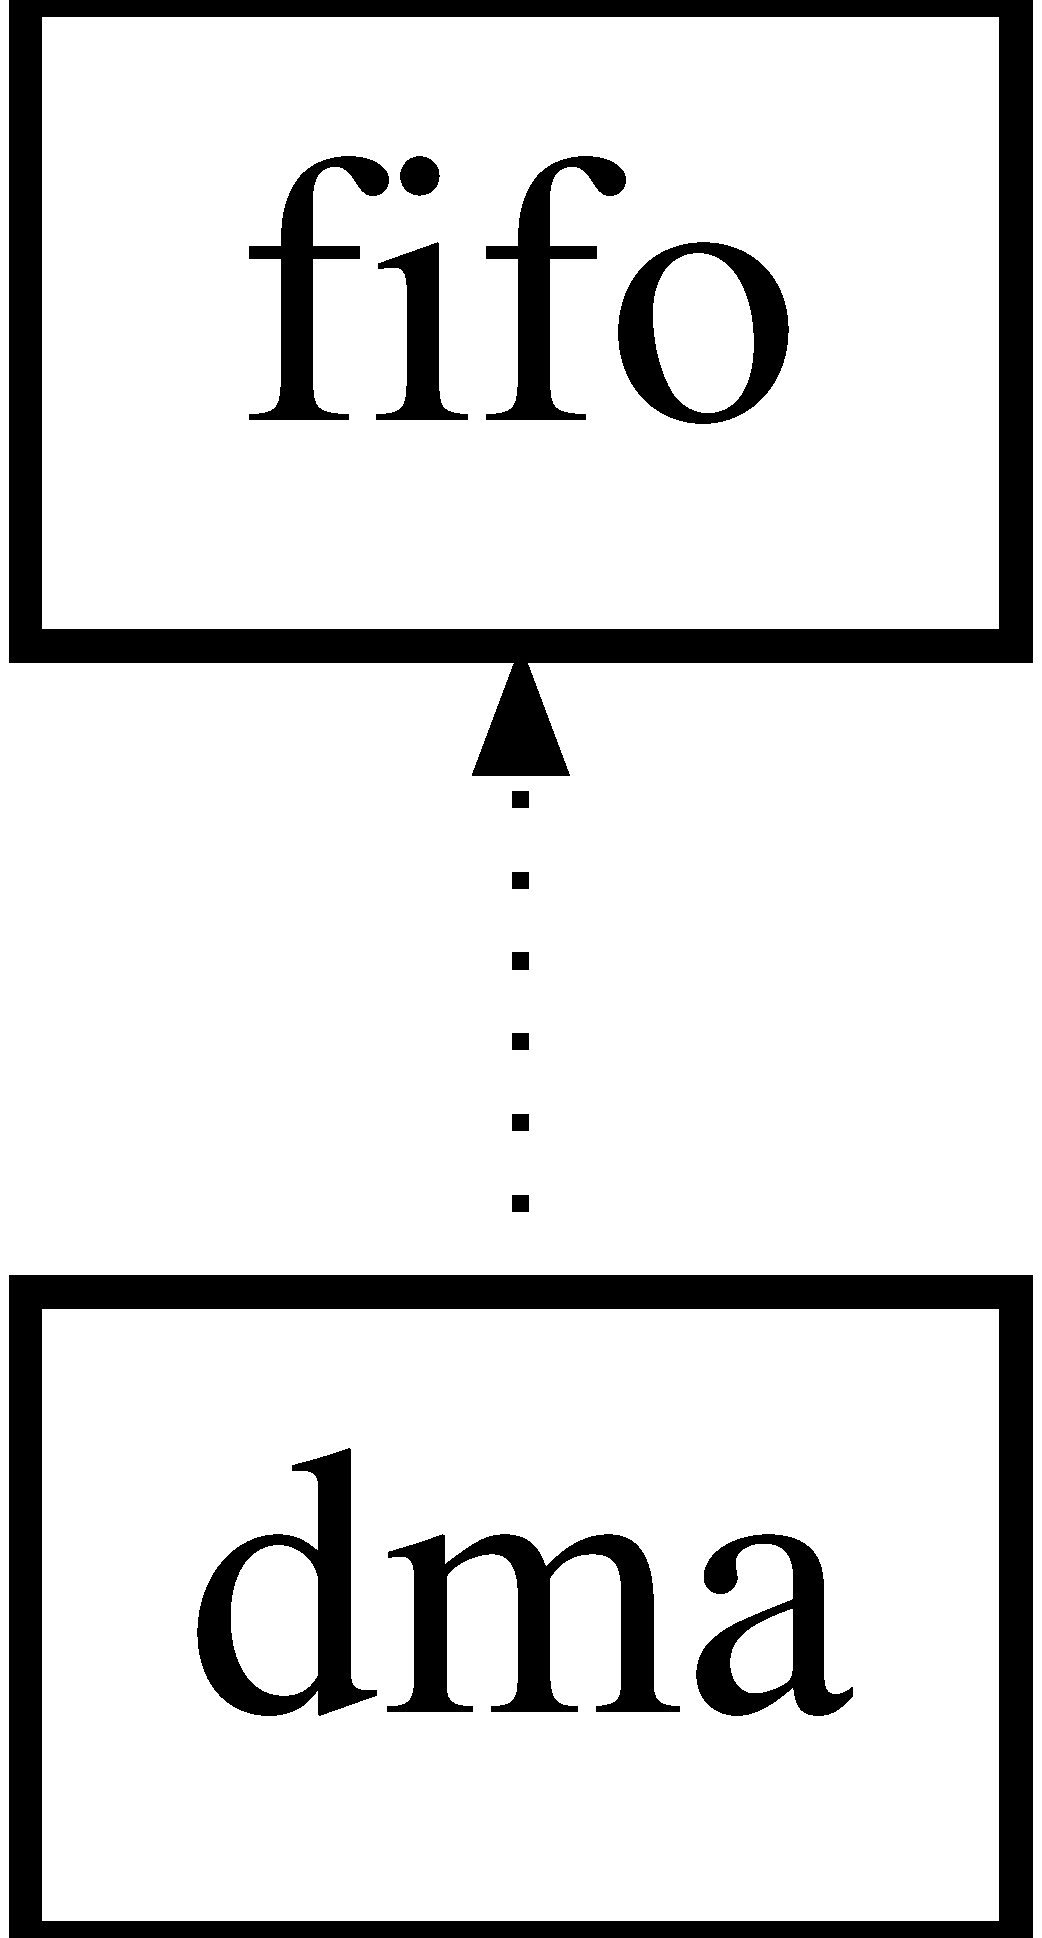
\includegraphics[height=2.000000cm]{d0/dcc/enumfifo}
\end{center}
\end{figure}
\begin{DoxyCompactItemize}
\item 
\mbox{\hyperlink{enumfifo_aa8122a479ce4de857afe9320219cfa5a}{A\+L\+W\+A\+Y\+S\+\_\+0}} rst
\begin{DoxyCompactList}\small\item\em Reset part. \end{DoxyCompactList}\item 
\mbox{\hyperlink{enumfifo_a45eb09cdeb334de587d997e4c9f2d6db}{A\+L\+W\+A\+Y\+S\+\_\+1}} clk
\begin{DoxyCompactList}\small\item\em Clock part. \end{DoxyCompactList}\end{DoxyCompactItemize}
\begin{DoxyCompactItemize}
\item 
\mbox{\hyperlink{enumfifo_ae0fe05859d03589d61cf0f69de9e7678}{clk}}
\begin{DoxyCompactList}\small\item\em clock input. \end{DoxyCompactList}\item 
\mbox{\hyperlink{enumfifo_a1cb4b0e761fcf0e2e1ff541d6af4ebad}{rst}}
\begin{DoxyCompactList}\small\item\em reset signal. The buffer will be set to 0 if reset. \end{DoxyCompactList}\item 
\mbox{\hyperlink{enumfifo_aaf4a37103205f6662b0a1d80a738adaa}{dir}}
\item 
\mbox{[}3\+:0\mbox{]} \mbox{\hyperlink{enumfifo_a0a60ca7138c275b0b4c6a99507b7f32b}{narrow\+\_\+port\+\_\+in}}
\item 
\mbox{[}7\+:0\mbox{]} \mbox{\hyperlink{enumfifo_afab6f412623dc4c22e9d8c6b98e847cd}{wide\+\_\+port\+\_\+in}}
\item 
reg \mbox{[}3\+:0\mbox{]} \mbox{\hyperlink{enumfifo_a94b95e7c8f83e2e7cb9865753d6bca50}{narrow\+\_\+port\+\_\+out}}
\item 
reg \mbox{[}7\+:0\mbox{]} \mbox{\hyperlink{enumfifo_aff07e3889d449c2cca44d3664a02aeaf}{wide\+\_\+port\+\_\+out}}
\item 
\mbox{\hyperlink{enumfifo_acfb9a73a88276cd8a16a0e77559171fc}{input\+\_\+valid}}
\item 
\mbox{\hyperlink{enumfifo_a2e34684dc888205692d0a1f9d4fbda76}{output\+\_\+enable}}
\item 
reg \mbox{\hyperlink{enumfifo_a6bbf9dd197f6264d333fe0505d8521eb}{input\+\_\+enable}}
\item 
reg \mbox{\hyperlink{enumfifo_a02360b908c47c6b5102e9597db8f51cb}{output\+\_\+valid}}
\item 
\mbox{\hyperlink{enumfifo_a5cb2b13451613d2af01db68febec6a50}{buffer}} reg\mbox{[}63\+:0\mbox{]}
\item 
\mbox{\hyperlink{enumfifo_aa0ade2ed497f56192af48cb015110e95}{width}} reg\mbox{[}56\+:0\mbox{]}
\item 
\mbox{\hyperlink{enumfifo_a5d5518c101413e893e36eb82384320c9}{narrow\+\_\+buffer}} reg\mbox{[}7\+:0\mbox{]}
\item 
\mbox{\hyperlink{enumfifo_a90a724159aa5f99c09e368ba5ed5f295}{narrow\+\_\+width}} reg\mbox{[}8\+:0\mbox{]}
\item 
\mbox{\hyperlink{enumfifo_a45c919098335b7a3b1089494455d9fcb}{direction}} reg
\end{DoxyCompactItemize}


\subsection{Detailed Description}
F\+I\+FO chip of fifferent data width with two directions. The direction will be determined when rst is set to 1. if direction is 0, data will be sent from narrow\+\_\+port to wide\+\_\+port, if direction is 1, the behavior is different. 

\subsection{Member Function Documentation}
\mbox{\Hypertarget{enumfifo_aa8122a479ce4de857afe9320219cfa5a}\label{enumfifo_aa8122a479ce4de857afe9320219cfa5a}} 
\index{fifo@{fifo}!A\+L\+W\+A\+Y\+S\+\_\+0@{A\+L\+W\+A\+Y\+S\+\_\+0}}
\index{A\+L\+W\+A\+Y\+S\+\_\+0@{A\+L\+W\+A\+Y\+S\+\_\+0}!fifo@{fifo}}
\subsubsection{\texorpdfstring{A\+L\+W\+A\+Y\+S\+\_\+0()}{ALWAYS\_0()}}
{\footnotesize\ttfamily  {\bfseries \textcolor{vhdlchar}{ }} A\+L\+W\+A\+Y\+S\+\_\+0(\begin{DoxyParamCaption}\item[{}]{{\bfseries \textcolor{vhdlchar}{rst}}   {\em {\bfseries \textcolor{vhdlchar}{ }}} }\end{DoxyParamCaption})\hspace{0.3cm}{\ttfamily [Always Construct]}}



Reset part. 

the reg direction will be set to the input dir. \mbox{\Hypertarget{enumfifo_a45eb09cdeb334de587d997e4c9f2d6db}\label{enumfifo_a45eb09cdeb334de587d997e4c9f2d6db}} 
\index{fifo@{fifo}!A\+L\+W\+A\+Y\+S\+\_\+1@{A\+L\+W\+A\+Y\+S\+\_\+1}}
\index{A\+L\+W\+A\+Y\+S\+\_\+1@{A\+L\+W\+A\+Y\+S\+\_\+1}!fifo@{fifo}}
\subsubsection{\texorpdfstring{A\+L\+W\+A\+Y\+S\+\_\+1()}{ALWAYS\_1()}}
{\footnotesize\ttfamily  {\bfseries \textcolor{vhdlchar}{ }} A\+L\+W\+A\+Y\+S\+\_\+1(\begin{DoxyParamCaption}\item[{}]{{\bfseries \textcolor{vhdlchar}{clk}}   {\em {\bfseries \textcolor{vhdlchar}{ }}} }\end{DoxyParamCaption})\hspace{0.3cm}{\ttfamily [Always Construct]}}



Clock part. 

if direction equals 1, narrow is input. if direction equals 0, wide is input. 

\subsection{Member Data Documentation}
\mbox{\Hypertarget{enumfifo_ae0fe05859d03589d61cf0f69de9e7678}\label{enumfifo_ae0fe05859d03589d61cf0f69de9e7678}} 
\index{fifo@{fifo}!clk@{clk}}
\index{clk@{clk}!fifo@{fifo}}
\subsubsection{\texorpdfstring{clk}{clk}}
{\footnotesize\ttfamily \mbox{\hyperlink{enumfifo_ae0fe05859d03589d61cf0f69de9e7678}{clk}} \hspace{0.3cm}{\ttfamily [Input]}}



clock input. 

\mbox{\Hypertarget{enumfifo_a1cb4b0e761fcf0e2e1ff541d6af4ebad}\label{enumfifo_a1cb4b0e761fcf0e2e1ff541d6af4ebad}} 
\index{fifo@{fifo}!rst@{rst}}
\index{rst@{rst}!fifo@{fifo}}
\subsubsection{\texorpdfstring{rst}{rst}}
{\footnotesize\ttfamily \mbox{\hyperlink{enumfifo_a1cb4b0e761fcf0e2e1ff541d6af4ebad}{rst}} \hspace{0.3cm}{\ttfamily [Input]}}



reset signal. The buffer will be set to 0 if reset. 

\mbox{\Hypertarget{enumfifo_aaf4a37103205f6662b0a1d80a738adaa}\label{enumfifo_aaf4a37103205f6662b0a1d80a738adaa}} 
\index{fifo@{fifo}!dir@{dir}}
\index{dir@{dir}!fifo@{fifo}}
\subsubsection{\texorpdfstring{dir}{dir}}
{\footnotesize\ttfamily \mbox{\hyperlink{enumfifo_aaf4a37103205f6662b0a1d80a738adaa}{dir}} \hspace{0.3cm}{\ttfamily [Input]}}

\mbox{\Hypertarget{enumfifo_a0a60ca7138c275b0b4c6a99507b7f32b}\label{enumfifo_a0a60ca7138c275b0b4c6a99507b7f32b}} 
\index{fifo@{fifo}!narrow\+\_\+port\+\_\+in@{narrow\+\_\+port\+\_\+in}}
\index{narrow\+\_\+port\+\_\+in@{narrow\+\_\+port\+\_\+in}!fifo@{fifo}}
\subsubsection{\texorpdfstring{narrow\+\_\+port\+\_\+in}{narrow\_port\_in}}
{\footnotesize\ttfamily \mbox{\hyperlink{enumfifo_a0a60ca7138c275b0b4c6a99507b7f32b}{narrow\+\_\+port\+\_\+in}} \hspace{0.3cm}{\ttfamily [Input]}}

\mbox{\Hypertarget{enumfifo_afab6f412623dc4c22e9d8c6b98e847cd}\label{enumfifo_afab6f412623dc4c22e9d8c6b98e847cd}} 
\index{fifo@{fifo}!wide\+\_\+port\+\_\+in@{wide\+\_\+port\+\_\+in}}
\index{wide\+\_\+port\+\_\+in@{wide\+\_\+port\+\_\+in}!fifo@{fifo}}
\subsubsection{\texorpdfstring{wide\+\_\+port\+\_\+in}{wide\_port\_in}}
{\footnotesize\ttfamily \mbox{\hyperlink{enumfifo_afab6f412623dc4c22e9d8c6b98e847cd}{wide\+\_\+port\+\_\+in}} \hspace{0.3cm}{\ttfamily [Input]}}

\mbox{\Hypertarget{enumfifo_a94b95e7c8f83e2e7cb9865753d6bca50}\label{enumfifo_a94b95e7c8f83e2e7cb9865753d6bca50}} 
\index{fifo@{fifo}!narrow\+\_\+port\+\_\+out@{narrow\+\_\+port\+\_\+out}}
\index{narrow\+\_\+port\+\_\+out@{narrow\+\_\+port\+\_\+out}!fifo@{fifo}}
\subsubsection{\texorpdfstring{narrow\+\_\+port\+\_\+out}{narrow\_port\_out}}
{\footnotesize\ttfamily \mbox{\hyperlink{enumfifo_a94b95e7c8f83e2e7cb9865753d6bca50}{narrow\+\_\+port\+\_\+out}} \hspace{0.3cm}{\ttfamily [Output]}}

\mbox{\Hypertarget{enumfifo_aff07e3889d449c2cca44d3664a02aeaf}\label{enumfifo_aff07e3889d449c2cca44d3664a02aeaf}} 
\index{fifo@{fifo}!wide\+\_\+port\+\_\+out@{wide\+\_\+port\+\_\+out}}
\index{wide\+\_\+port\+\_\+out@{wide\+\_\+port\+\_\+out}!fifo@{fifo}}
\subsubsection{\texorpdfstring{wide\+\_\+port\+\_\+out}{wide\_port\_out}}
{\footnotesize\ttfamily \mbox{\hyperlink{enumfifo_aff07e3889d449c2cca44d3664a02aeaf}{wide\+\_\+port\+\_\+out}} \hspace{0.3cm}{\ttfamily [Output]}}

\mbox{\Hypertarget{enumfifo_acfb9a73a88276cd8a16a0e77559171fc}\label{enumfifo_acfb9a73a88276cd8a16a0e77559171fc}} 
\index{fifo@{fifo}!input\+\_\+valid@{input\+\_\+valid}}
\index{input\+\_\+valid@{input\+\_\+valid}!fifo@{fifo}}
\subsubsection{\texorpdfstring{input\+\_\+valid}{input\_valid}}
{\footnotesize\ttfamily \mbox{\hyperlink{enumfifo_acfb9a73a88276cd8a16a0e77559171fc}{input\+\_\+valid}} \hspace{0.3cm}{\ttfamily [Input]}}

\mbox{\Hypertarget{enumfifo_a2e34684dc888205692d0a1f9d4fbda76}\label{enumfifo_a2e34684dc888205692d0a1f9d4fbda76}} 
\index{fifo@{fifo}!output\+\_\+enable@{output\+\_\+enable}}
\index{output\+\_\+enable@{output\+\_\+enable}!fifo@{fifo}}
\subsubsection{\texorpdfstring{output\+\_\+enable}{output\_enable}}
{\footnotesize\ttfamily \mbox{\hyperlink{enumfifo_a2e34684dc888205692d0a1f9d4fbda76}{output\+\_\+enable}} \hspace{0.3cm}{\ttfamily [Input]}}

\mbox{\Hypertarget{enumfifo_a6bbf9dd197f6264d333fe0505d8521eb}\label{enumfifo_a6bbf9dd197f6264d333fe0505d8521eb}} 
\index{fifo@{fifo}!input\+\_\+enable@{input\+\_\+enable}}
\index{input\+\_\+enable@{input\+\_\+enable}!fifo@{fifo}}
\subsubsection{\texorpdfstring{input\+\_\+enable}{input\_enable}}
{\footnotesize\ttfamily \mbox{\hyperlink{enumfifo_a6bbf9dd197f6264d333fe0505d8521eb}{input\+\_\+enable}} \hspace{0.3cm}{\ttfamily [Output]}}

\mbox{\Hypertarget{enumfifo_a02360b908c47c6b5102e9597db8f51cb}\label{enumfifo_a02360b908c47c6b5102e9597db8f51cb}} 
\index{fifo@{fifo}!output\+\_\+valid@{output\+\_\+valid}}
\index{output\+\_\+valid@{output\+\_\+valid}!fifo@{fifo}}
\subsubsection{\texorpdfstring{output\+\_\+valid}{output\_valid}}
{\footnotesize\ttfamily \mbox{\hyperlink{enumfifo_a02360b908c47c6b5102e9597db8f51cb}{output\+\_\+valid}} \hspace{0.3cm}{\ttfamily [Output]}}

\mbox{\Hypertarget{enumfifo_a5cb2b13451613d2af01db68febec6a50}\label{enumfifo_a5cb2b13451613d2af01db68febec6a50}} 
\index{fifo@{fifo}!buffer@{buffer}}
\index{buffer@{buffer}!fifo@{fifo}}
\subsubsection{\texorpdfstring{buffer}{buffer}}
{\footnotesize\ttfamily \mbox{\hyperlink{enumfifo_a5cb2b13451613d2af01db68febec6a50}{buffer}} \hspace{0.3cm}{\ttfamily [Signal]}}

\mbox{\Hypertarget{enumfifo_aa0ade2ed497f56192af48cb015110e95}\label{enumfifo_aa0ade2ed497f56192af48cb015110e95}} 
\index{fifo@{fifo}!width@{width}}
\index{width@{width}!fifo@{fifo}}
\subsubsection{\texorpdfstring{width}{width}}
{\footnotesize\ttfamily \mbox{\hyperlink{enumfifo_aa0ade2ed497f56192af48cb015110e95}{width}} \hspace{0.3cm}{\ttfamily [Signal]}}

\mbox{\Hypertarget{enumfifo_a5d5518c101413e893e36eb82384320c9}\label{enumfifo_a5d5518c101413e893e36eb82384320c9}} 
\index{fifo@{fifo}!narrow\+\_\+buffer@{narrow\+\_\+buffer}}
\index{narrow\+\_\+buffer@{narrow\+\_\+buffer}!fifo@{fifo}}
\subsubsection{\texorpdfstring{narrow\+\_\+buffer}{narrow\_buffer}}
{\footnotesize\ttfamily \mbox{\hyperlink{enumfifo_a5d5518c101413e893e36eb82384320c9}{narrow\+\_\+buffer}} \hspace{0.3cm}{\ttfamily [Signal]}}

\mbox{\Hypertarget{enumfifo_a90a724159aa5f99c09e368ba5ed5f295}\label{enumfifo_a90a724159aa5f99c09e368ba5ed5f295}} 
\index{fifo@{fifo}!narrow\+\_\+width@{narrow\+\_\+width}}
\index{narrow\+\_\+width@{narrow\+\_\+width}!fifo@{fifo}}
\subsubsection{\texorpdfstring{narrow\+\_\+width}{narrow\_width}}
{\footnotesize\ttfamily \mbox{\hyperlink{enumfifo_a90a724159aa5f99c09e368ba5ed5f295}{narrow\+\_\+width}} \hspace{0.3cm}{\ttfamily [Signal]}}

\mbox{\Hypertarget{enumfifo_a45c919098335b7a3b1089494455d9fcb}\label{enumfifo_a45c919098335b7a3b1089494455d9fcb}} 
\index{fifo@{fifo}!direction@{direction}}
\index{direction@{direction}!fifo@{fifo}}
\subsubsection{\texorpdfstring{direction}{direction}}
{\footnotesize\ttfamily \mbox{\hyperlink{enumfifo_a45c919098335b7a3b1089494455d9fcb}{direction}} \hspace{0.3cm}{\ttfamily [Signal]}}



The documentation for this module was generated from the following file\+:\begin{DoxyCompactItemize}
\item 
Final\+Elec.\+srcs/sources\+\_\+1/new/\mbox{\hyperlink{fifo_8v}{fifo.\+v}}\end{DoxyCompactItemize}

\chapter{File Documentation}
\hypertarget{dma_8v}{}\section{Final\+Elec.\+srcs/sources\+\_\+1/new/dma.v File Reference}
\label{dma_8v}\index{Final\+Elec.\+srcs/sources\+\_\+1/new/dma.\+v@{Final\+Elec.\+srcs/sources\+\_\+1/new/dma.\+v}}
\subsection*{Classes}
\begin{DoxyCompactItemize}
\item 
Module \mbox{\hyperlink{enumdma}{dma}}
\end{DoxyCompactItemize}
\begin{DoxyCompactItemize}
\item 
include \mbox{\hyperlink{dma_8v_a1e5c1a4f3cd875bdef06967cc860334a}{fifo.\+v}}
\end{DoxyCompactItemize}


\subsection{Variable Documentation}
\mbox{\Hypertarget{dma_8v_a1e5c1a4f3cd875bdef06967cc860334a}\label{dma_8v_a1e5c1a4f3cd875bdef06967cc860334a}} 
\index{dma.\+v@{dma.\+v}!fifo.\+v@{fifo.\+v}}
\index{fifo.\+v@{fifo.\+v}!dma.\+v@{dma.\+v}}
\subsubsection{\texorpdfstring{fifo.\+v}{fifo.v}}
{\footnotesize\ttfamily \mbox{\hyperlink{dma_8v_a1e5c1a4f3cd875bdef06967cc860334a}{fifo.\+v}} \hspace{0.3cm}{\ttfamily [Include]}}


\hypertarget{fifo_8v}{}\section{Final\+Elec.\+srcs/sources\+\_\+1/new/fifo.v File Reference}
\label{fifo_8v}\index{Final\+Elec.\+srcs/sources\+\_\+1/new/fifo.\+v@{Final\+Elec.\+srcs/sources\+\_\+1/new/fifo.\+v}}


First in first out memory module.  


\subsection*{Classes}
\begin{DoxyCompactItemize}
\item 
Module \mbox{\hyperlink{enumfifo}{fifo}}
\end{DoxyCompactItemize}


\subsection{Detailed Description}
First in first out memory module. 

\begin{DoxyAuthor}{Author}
Liu Shiqi\href{mailto:liushiqi17@mails.ucas.ac.cn}{\tt liushiqi17@mails.\+ucas.\+ac.\+cn}, Li Feidong 
\end{DoxyAuthor}
\begin{DoxyVersion}{Version}
0.\+1.\+0 
\end{DoxyVersion}
\begin{DoxyDate}{Date}
2019-\/01-\/08 
\end{DoxyDate}

%--- End generated contents ---

% Index
\backmatter
\newpage
\phantomsection
\clearemptydoublepage
\addcontentsline{toc}{chapter}{Index}
\printindex

\end{document}
